
\documentclass[tikz,convert={outfile=\jobname.png}]{standalone}

\usepackage[utf8]{inputenc}
\usepackage{tikz}
\usepackage{pgfplots}
\pgfplotsset{compat=newest}
\usepgfplotslibrary{groupplots}
\begin{document}
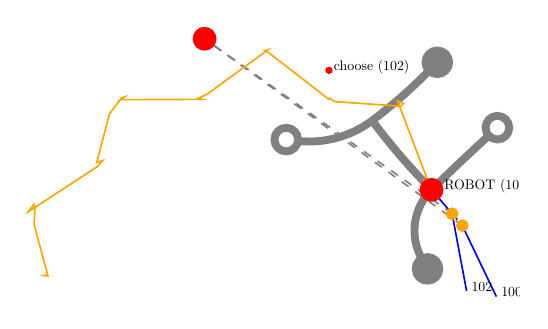
\begin{tikzpicture}[scale=1]
\def\col{gray}
\def\lw{1mm}
\def\alpi{2.000000}
\def\beti{74.723709}
\def\gam{-7.637894}
\def\alpii{8.768087}
\def\betii{43.107456}
\def\gamh{-3.818947}
\def\eps{-49.364207}
\def\ci{-47.514981}
\def\cii{29.178449}
\def\ciii{135.584933}
\def\civ{83.709390}
\def\ri{28.648050}
\def\rii{0.727397}
\def\rg{-8.697878}
\def\riii{6.285329}
\def\riv{1.329109}
\path (5.608369, 1.769428)coordinate(F1);
\draw[\col, line width=\lw] (F1)arc(180+\ci:180+\ci+\alpi:\ri)coordinate(OM);
\draw[\col, line width=\lw] (OM)arc(180+\ci+\alpi:180+\ci+\alpi+\beti:\rii)coordinate(F2);
\draw[\col, line width=\lw] (OM)arc(90+\ci+\alpi:90+\ci+\alpi+\gam:\rg)coordinate(UM);
\draw[\col, line width=\lw] (UM)arc(\gam+\ci+\alpi:\gam+\ci+\alpi+\alpii:\riii)coordinate(F3);
\draw[\col, line width=\lw] (UM)arc(\gam+\ci+\alpi:\gam+\ci+\alpi-\betii:\riv)coordinate(F4);
\draw[\col, line width=\lw] (F1)++(42.485019 :.15) circle(.15);
\draw[\col, line width=\lw, fill] (F2)++(-60.821551 :.15) circle(.15);
\draw[\col, line width=\lw, fill] (F3)++(45.584933 :.15) circle(.15);
\draw[\col, line width=\lw] (F4)++(173.709390 :.15) circle(.15);
% This file was created by matplotlib2tikz v0.7.4.
\definecolor{color0}{rgb}{1,0.647058823529412,0}
\begin{axis}[
anchor=origin,
disabledatascaling,
hide x axis,
hide y axis,
tick align=outside,
tick pos=left,
x grid style={white!69.01960784313725!black},
x=1cm,
xmin=-0.533367802531329, xmax=6.0031780217287,
xtick style={color=black},
y grid style={white!69.01960784313725!black},
y=1cm,
ymin=-0.439166215039552, ymax=3.16376981976379,
ytick style={color=black}
]
\addplot [semithick, red, mark=*, mark size=4, mark options={solid}]
table {%
4.88266421384587 1.08148480042251
};
\addplot [semithick, blue]
table {%
4.88266421384587 1.08148480042251
5.20828841880278 0.702052491378875
};
\addplot [semithick, red, mark=*, mark size=1, mark options={solid}]
table {%
4.88266421384587 1.08148480042251
};
\addplot [semithick, blue]
table {%
4.88266421384587 1.08148480042251
4.98266421384587 1.08148480042251
};
\addplot [semithick, red, mark=*, mark size=4, mark options={solid}]
table {%
2 3
};
\addplot [semithick, blue]
table {%
2 3
2 3
};
\addplot [semithick, color0, mark=*, mark size=2, mark options={solid}]
table {%
5.14316357781139 0.777938953187602
};
\addplot [semithick, blue]
table {%
5.14316357781139 0.777938953187602
5.32772893592734 -0.204881289066053
};
\addplot [semithick, white!50.19607843137255!black, dashed]
table {%
5.14316357781139 0.777938953187602
2 3
};
\addplot [semithick, color0, mark=*, mark size=2, mark options={solid}]
table {%
5.27341325979416 0.626166029570148
};
\addplot [semithick, blue]
table {%
5.27341325979416 0.626166029570148
5.70606230244415 -0.275396395275764
};
\addplot [semithick, white!50.19607843137255!black, dashed]
table {%
5.27341325979416 0.626166029570148
2 3
};
\addplot [semithick, red, mark=*, mark size=1, mark options={solid}]
table {%
3.58016739401826 2.59921403659705
};
\addplot [semithick, blue]
table {%
3.58016739401826 2.59921403659705
3.58016739401826 2.59921403659705
};
\addplot [semithick, color0]
table {%
2.22044604925031e-16 0
-0.035284306538821 -0.00829016687913958
0.0104823285577833 -0.0115319758319767
-0.164252533096797 0.637677398262343
-0.154535150830559 0.856696082853981
-0.169243463423073 0.896607412910113
-0.236252083246782 0.80462614580702
0.634841878140266 1.37354801115764
0.705884564575145 1.45347461847376
0.62975361853255 1.43005620418242
0.792894272810572 2.04712327676978
0.946823170367455 2.24906227825262
0.977765820964178 2.25850997466114
0.932218039751831 2.22618466667364
1.97140548117453 2.2303302654593
1.92021430259214 2.24284119193837
2.03761254623753 2.29961236448717
2.80613394800623 2.86043950709798
2.76819466602352 2.85108256996867
2.78866478253126 2.84148627334007
3.57600905812447 2.23308524468796
3.59175721110567 2.24293828012203
3.65594266441652 2.20157240781185
4.48813549645312 2.14321921489002
4.52571107612275 2.17600499577973
4.45079267639025 2.20995279635902
4.85562290641024 1.14148110593298
4.77810040697537 1.20889324860187
4.88266421384587 1.08148480042251
};
\node at (axis cs:4.98266421384587,1.08148480042251)[
  scale=0.5,
  anchor=base west,
  text=black,
  rotate=0.0
]{ROBOT (103df)};
\node at (axis cs:5.32772893592734,-0.204881289066053)[
  scale=0.5,
  anchor=base west,
  text=black,
  rotate=0.0
]{102};
\node at (axis cs:5.70606230244415,-0.275396395275764)[
  scale=0.5,
  anchor=base west,
  text=black,
  rotate=0.0
]{100};
\node at (axis cs:3.58016739401826,2.59921403659705)[
  scale=0.5,
  anchor=base west,
  text=black,
  rotate=0.0
]{choose (102)};
\end{axis}
\end{tikzpicture}
%% End matplotlib2tikz content %% 
\end{document}